\documentclass[11pt]{article}
\usepackage[margin=1in]{geometry}
\usepackage{amsmath,amssymb}
\usepackage{enumitem}
\usepackage{multicol}
\usepackage{tikz}
\usepackage{pgfplots}
\pgfplotsset{compat=1.17}
\usepackage{array}
\usepackage{booktabs}
\usepackage{titlesec}
\usepackage{tcolorbox}
\usepackage{fancyhdr}

% ---------- Custom commands for better fill-ins ----------
\newcommand{\fillin}[1][2.25in]{\makebox[#1]{\hrulefill}}
\newcommand{\shortfill}[1][1in]{\makebox[#1]{\hrulefill}}
\newcommand{\mediumfill}[1][1.5in]{\makebox[#1]{\hrulefill}}
\newcommand{\longfill}[1][4in]{\makebox[#1]{\hrulefill}}
\newcommand{\linespace}{\vspace{0.8\baselineskip}}
\newcommand{\checkbox}{$\square$}

% ---------- Better list formatting ----------
\setlist[itemize]{leftmargin=1.1em, noitemsep, topsep=3pt}
\setlist[enumerate]{leftmargin=1.4em, noitemsep, topsep=3pt}

% ---------- Section formatting ----------
\titleformat{\section}{\large\bfseries}{\thesection}{0.5em}{}
\titleformat{\subsection}{\normalsize\bfseries}{\thesubsection}{0.5em}{}

% Header setup
\pagestyle{fancy}
\fancyhf{}
\lhead{AP Statistics - Unit 2.4}
\rhead{Video 2: Bivariate Data}
\cfoot{Page \thepage}

\begin{document}

\begin{center}
    {\Large \textbf{AP Statistics Unit 2.4, Video 2}}\\[0.2em]
    {\large Sentence Frame Worksheet: Bivariate Data \& Scatter Plots}\\[0.3em]
    \textit{Mr. Youngsaver - College Board}
\end{center}

\noindent
\textbf{Name:} \longfill \hfill 
\textbf{Date:} \mediumfill \hfill 
\textbf{Period:} \shortfill

\section*{Learning Targets}
\textit{Fill in as you watch the video introduction (00:00--00:28)}
\begin{itemize}
    \item I can distinguish between \fillin[1.8in] and \fillin[1.8in] variables
    \item I can determine which variable is plotted on the \shortfill[0.8in]-axis and which on the \shortfill[0.8in]-axis
    \item I can construct a \fillin[1.5in] with proper title, labels, and scale
\end{itemize}

\section*{Key Vocabulary}
\textit{Complete definitions as terms are introduced in the video}

\begin{multicols}{2}
\begin{enumerate}
    \item \textbf{Explanatory variable:} \longfill[2in] \\
    \fillin[2.3in] \\
    (also called the \shortfill[0.8in] variable)
    
    \item \textbf{Response variable:} \longfill[2in] \\
    \fillin[2.3in] \\
    (also called the \shortfill[0.8in] variable)
    
    \item \textbf{Bivariate data:} \longfill[2in] \\
    \fillin[2.3in]
    
    \item \textbf{Scatter plot:} \longfill[2in] \\
    \fillin[2.3in]
\end{enumerate}
\end{multicols}

\section*{Video Notes by Section}

\subsection*{Part 1: Context \& Critical Thinking (00:31--01:19)}

\begin{tcolorbox}[colback=blue!5,colframe=blue!40!black,title=The Income Achievement Gap]
\begin{enumerate}[label=\alph*)]
    \item In the U.S., \mediumfill and \mediumfill-income students tend to perform \fillin[1.2in] on math exams than \fillin[1.2in]-income students \textbf{on average}.
    
    \item \textbf{CRITICAL NOTE:} This data says \fillin[1.5in] about individual performance or intelligence. It only shows trends of \fillin[1.3in] for full groups.
\end{enumerate}
\end{tcolorbox}

\subsection*{Part 2: The Attendance Connection (01:53--03:05)}

\begin{enumerate}[label=\alph*)]
    \item There's also an "income \fillin[1.3in] gap" where higher-income areas have \fillin[1.2in] chronically absent students.
    
    \item Two possible reasons mentioned:
    \begin{enumerate}[label=(\arabic*)]
        \item \longfill[3.5in]
        \item \longfill[3.5in]
    \end{enumerate}
    
    \item The key question: If we improve \fillin[1.5in] for lower-income students, will their \fillin[1.8in] also improve?
\end{enumerate}

\subsection*{Part 3: Identifying Variables (03:11--03:58)}

\begin{tcolorbox}[colback=yellow!10,colframe=orange!60!black,title=The Example Data]
Sample size: \shortfill[0.5in] students\\[0.3em]
Two variables measured:
\begin{itemize}
    \item Variable 1: \longfill[3in]
    \item Variable 2: \longfill[3in]
\end{itemize}
\end{tcolorbox}

\textbf{Complete this reasoning:}\\
"We think \fillin[2in] might help explain or predict \fillin[2in]."\\[0.3em]
Therefore:
\begin{itemize}
    \item The \textbf{explanatory} variable (X) is: \fillin[2.5in]
    \item The \textbf{response} variable (Y) is: \fillin[2.5in]
\end{itemize}

\begin{tcolorbox}[colback=green!10,colframe=green!40!black,title=Memory Trick]
e\textbf{X}planatory = \shortfill[0.5in] variable\\
Response = \shortfill[0.5in] variable
\end{tcolorbox}

\subsection*{Part 4: Creating the Scatter Plot (04:08--05:11)}

\textbf{When to use a scatter plot:}
\begin{itemize}
    \item Number of variables: \shortfill[0.5in]
    \item Type of variables: Both must be \fillin[1.5in] (not categorical)
\end{itemize}

\textbf{Essential components of a quality scatter plot:}
\begin{enumerate}
    \item \longfill[4in]
    \item \longfill[4in]
    \item \longfill[4in]
\end{enumerate}

\section*{Variable Analysis Table}
\textit{Complete for the video's example}

\begin{center}
\begin{tabular}{|l|p{3.5cm}|p{3.5cm}|}
\hline
\textbf{Characteristic} & \textbf{Variable 1} & \textbf{Variable 2} \\
\hline
Name & \fillin[3cm] & \fillin[3cm] \\
\hline
Units & \fillin[3cm] & \fillin[3cm] \\
\hline
Type (categorical/quantitative) & \fillin[3cm] & \fillin[3cm] \\
\hline
Role (explanatory/response) & \fillin[3cm] & \fillin[3cm] \\
\hline
Axis placement (X or Y) & \fillin[3cm] & \fillin[3cm] \\
\hline
\multicolumn{3}{|l|}{\textbf{Reasoning:} Why does Variable 1 explain Variable 2?} \\
\multicolumn{3}{|p{14cm}|}{\vspace{0.2cm}\longfill[13cm]\vspace{0.2cm}} \\
\hline
\end{tabular}
\end{center}

\section*{Construct Your Scatter Plot}

\textbf{Planning:}
\begin{itemize}
    \item Title: \longfill[4in]
    \item X-axis range: from \shortfill[0.8in] to \shortfill[0.8in], tick marks every \shortfill[0.8in]
    \item Y-axis range: from \shortfill[0.8in] to \shortfill[0.8in], tick marks every \shortfill[0.8in]
\end{itemize}

\begin{center}
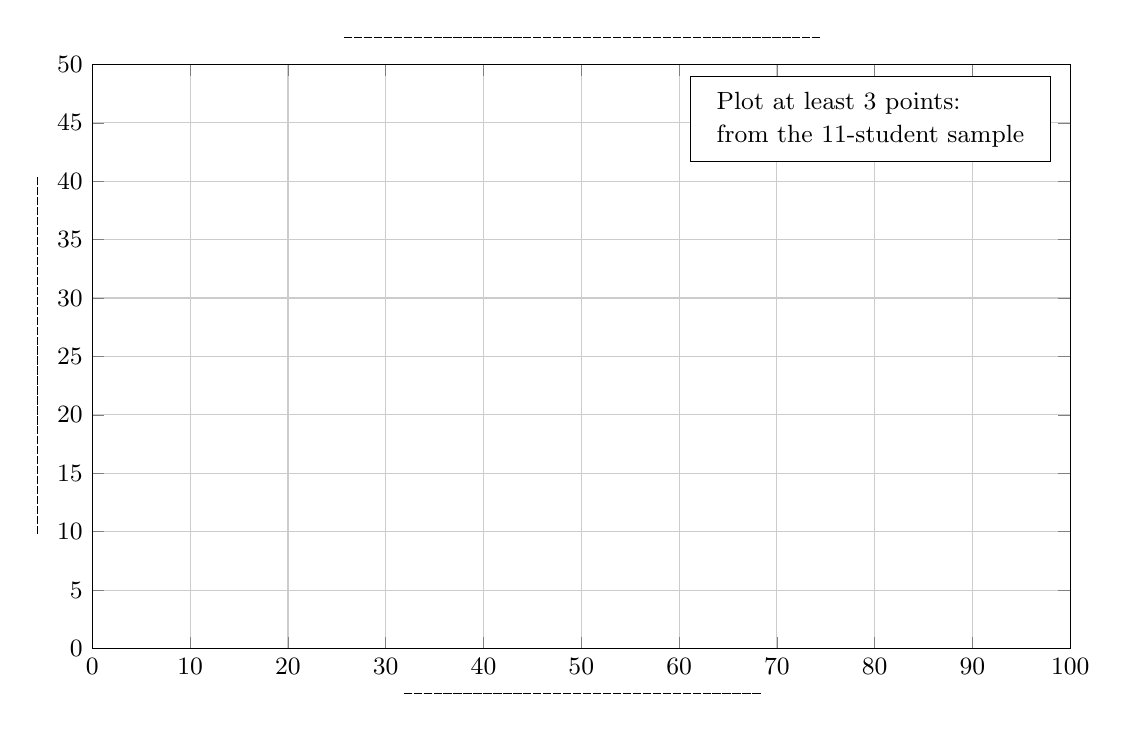
\begin{tikzpicture}
\begin{axis}[
    width=14cm,
    height=9cm,
    xlabel={\_\_\_\_\_\_\_\_\_\_\_\_\_\_\_\_\_\_\_\_\_\_\_\_\_\_\_\_\_\_\_\_\_\_\_\_},
    ylabel={\_\_\_\_\_\_\_\_\_\_\_\_\_\_\_\_\_\_\_\_\_\_\_\_\_\_\_\_\_\_\_\_\_\_\_\_},
    xmin=0, xmax=100,
    ymin=0, ymax=50,
    grid=both,
    grid style={line width=0.2pt, draw=gray!20},
    major grid style={line width=0.4pt,draw=gray!40},
    title={\_\_\_\_\_\_\_\_\_\_\_\_\_\_\_\_\_\_\_\_\_\_\_\_\_\_\_\_\_\_\_\_\_\_\_\_\_\_\_\_\_\_\_\_\_\_\_\_},
    xlabel style={font=\normalsize},
    ylabel style={font=\normalsize},
    xtick={0,10,20,30,40,50,60,70,80,90,100},
    ytick={0,5,10,15,20,25,30,35,40,45,50},
    tick label style={font=\small}
]
% Students plot points here
% Add note box for students
\node[draw, fill=white, anchor=north east] at (rel axis cs:0.98,0.98) {
    \begin{tabular}{l}
    \small Plot at least 3 points:\\
    \small from the 11-student sample
    \end{tabular}
};
\end{axis}
\end{tikzpicture}
\end{center}

\section*{Quality Self-Check}
\textit{Check off each item when your scatter plot is complete:}
\begin{itemize}
    \item \checkbox\, My graph has a descriptive \fillin[1in] that includes context
    \item \checkbox\, Both axes are clearly \fillin[1in] with variable names and units
    \item \checkbox\, The scale has appropriate \fillin[1.2in] marks that aren't misleading
    \item \checkbox\, Each point represents one \fillin[1.2in] with (x,y) coordinates
    \item \checkbox\, The explanatory variable is on the \shortfill[0.5in]-axis
    \item \checkbox\, The response variable is on the \shortfill[0.5in]-axis
\end{itemize}

\section*{Looking Ahead (05:14--05:30)}
\textit{Without using technical terms yet, describe patterns you notice:}
\begin{enumerate}
    \item Overall trend I see: \longfill[4.5in]
    \item Unusual features: \longfill[4.5in]
    \item Words to describe the pattern: \fillin[1in], \fillin[1in], \fillin[1in]
\end{enumerate}

\section*{The Statistician's Code (05:50--05:59)}
According to Mr. Youngsaver, statisticians should:
\begin{itemize}
    \item Be \fillin[1.2in]
    \item Be \fillin[1.2in]
    \item Be \fillin[1.2in]
    \item Avoid \shortfill[0.8in] (which stands for \fillin[1.8in])
\end{itemize}

\section*{Exit Ticket}
\textit{Complete before leaving class:}
\begin{enumerate}
    \item In your own words: The \fillin[1.5in] variable helps explain or predict the \fillin[1.5in] variable. We place the first on the \shortfill[0.5in]-axis and the second on the \shortfill[0.5in]-axis.
    
    \item Three essential elements every scatter plot needs:
    \begin{enumerate}[label=\arabic*)]
        \item \fillin[3in]
        \item \fillin[3in]
        \item \fillin[3in]
    \end{enumerate}
    
    \item Why is it important to identify which variable is explanatory vs. response before creating a scatter plot?\\
    \longfill[5in]\\
    \longfill[5in]
\end{enumerate}

\section*{Challenge Extension}
\textit{Optional: Create your own example}

Think of two quantitative variables from your life where one might explain the other:
\begin{itemize}
    \item My explanatory variable: \fillin[2.5in]
    \item My response variable: \fillin[2.5in]
    \item Why this relationship makes sense: \longfill[4in]\\
    \longfill[5in]
\end{itemize}

\vfill
\hrule
\small
\noindent
\textit{Note:} Fill each blank with precise language from the video. Use specific context (variable names, units) whenever possible. This worksheet covers Video 2 of Unit 2.4 presented by Mr. Youngsaver from the College Board AP Statistics team.

\end{document}